\setAuthor{Valter Kiisk}
\setRound{piirkonnavoor}
\setYear{2018}
\setNumber{G 8}
\setDifficulty{5}
\setTopic{Elektriahelad}

\prob{12 lampi}
Juku käsutuses on 12 ühesugust taskulambipirni ning patarei, mille klemmipinge on täpselt 5 korda suurem pirni nimipingest. Lisaks leidis ta juhtumisi takisti, mille takistus on parajasti pool lambi hõõgniidi takistusest töörežiimis (viimase sai ta teada jagades lambi soklile kirjutatud nimipinge ja -voolu omavahel).\\
\osa Kuidas tuleb ühendada nimetatud komponendid elektriahelasse, et kõik 12 pirni põleksid normaalheledusega?\\
\osa Mitu korda kasvab (või kahaneb) lampide koguvõimsus, kui üks lampidest läbi põleb? Lampide takistuse sõltuvust temperatuurist võib jätta arvestamata.

\hint
Eesmärk on leida elektriskeem, kus igale lambile langeb viiendik klemmipingest. Mõistlik on kõigepealt proovida võimalikult lihtsaid korrapäraseid lampide konfiguratsioone. Näiteks saab lambid asetada rööpühendusse, kus igas harus on kas 1, 2, 3, 4, 6 või 12 lampi.

\solu
\osa Ilmselt tuleb takisti voolu piiramiseks ühendada järjestikku vooluallikaga (ükski teine kombinatsioon, sh takisti ärajätmine, ei võimalda kõiki 12 lampi lülitada nominaalpingele). Lambid saab põhimõtteliselt ahelasse ühendada 1-, 2-, 3-, 4-, 6- või 12-kaupa jadamisi ja seejärel rööbiti (st kõik lambid on ahelasse lülitatud ühetaoliselt). Iga kombinatsiooni korral arvutame esmalt ahela erinevate osade takistuse (ühikutes $R$, mis on üksiku lambi takistus) ja seejärel arvestame pinge jagunemist elementidel proportsionaalselt takistusega. Erinevate variantide kontrollimine näitab, et lambile langeb nominaalpinge näiteks juhul, kui ühendada lambid kahekaupa jadamisi ja seejärel 6 sellist ahelat rööbiti. Seega, õige skeem on selline, nagu kujutatud joonisel.

\begin{center}
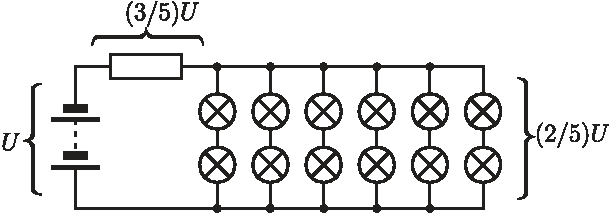
\includegraphics{2018-v2g-08-lambid-joonis.pdf}
\end{center}

Kuni kõik lambid põlevad, langeb igale lambile pinge $U/5$, kus $U$ on pingeallika klemmipinge. Koguvõimsus on vastavalt
\[
P_1=12\times \frac{U^2}{25R}=\frac{12U^2}{25R},
\]
kus $R$ on üksiku lambi takistus. Kui üks lampidest põleb läbi, siis ka sellega järjestikku ühendatud pirn lõpetab töötamise. Järele jääb vaid 5 rööbiti ühendatud ahelat ja seega lampide kogutakistus on $2R/5$. Võttes nüüd arvesse pinge jagunemist ahelas, saab pinge igal lambil olema
\[
U\times \frac{2R/5}{2R/5+R/2} \times \frac{1}{2}=\frac{2}{9}U
\]
ja lampide koguvõimsus vastavalt
\[
P_2=10\times \frac{4U^2}{81R}=\frac{40U^2}{81R}.
\]
Seega koguvõimsus kasvab $P_2/P_1=250/243\approx \num{1.029}$ korda.

\textit{Märkus.} Leidub veel mitu sobivat skeemi. Toome mõned neist.
\begin{itemize} 
\item
Ühendame lambid kolmekaupa jadamisi ja seejärel 4 sellist ahelat rööbiti. Sel juhul osas \textit{b)} kahaneb lampide koguvõimsus $\num{1.080}$ korda.
\item
Ühendame lambid neljakaupa rööbiti ja seejärel 3 sellist plokki jadamisi takistiga. Sel juhul osas \textit{b)} kahaneb lampide koguvõimsus $\num{1.024}$ korda
\end{itemize}
Töötavaid skeeme leidub rohkemgi.

\probeng{12 Lamps}
Juku has 12 identical flashlight’s bulbs and a battery. The voltage on the battery’s leads is exactly 5 times bigger than the bulb’s nominal voltage. Juku also found a resistor which has a resistance two times smaller than the resistance of the bulb’s filament in working regimen (the latter was found by dividing the nominal voltage written on the bulb’s socle by the nominal current written on it).\\
\osa How must be the mentioned components connected to a circuit diagram so that all the 12 light bulbs operate with nominal brightness?\\
\osa How many times will the total power of the lights increase (or decrease) if one of the bulbs fuses? Do not account for the relation between the resistance of the lamps and the temperature.

\hinteng
The goal is to find a circuit where one fifth of voltage on the leads is applied to each lamp. It would be reasonable to first try configurations as simple as possible for ordered lamps. For example the lamps can be connected in parallel where each branch has either 1, 2, 3, 4, 6 or 12 lamps.

\solueng
a) The resistor would probably have to be connected sequentially to a current source to limit the current (no other combination, including leaving out the resistor, does not allow all the 12 lamps to work on a nominal voltage). The lamps can fundamentally be connected in series by 1, 2, 3, 4, 6 or 12 and then in parallel (meaning that all the lamps are connected in the same way in the diagram). For each combination let us first calculate the resistance of the diagram’s different parts (in the units $R$, which is the resistance of one lamp) and then we consider the distribution of the voltage to the elements proportionally with resistance. Checking different options shows that a lamp would have nominal voltage in the case where the lamps are connected in series by 2 and then 6 such series are connected in parallel. Therefore the correct diagram is such as in the figure.
\begin{center}
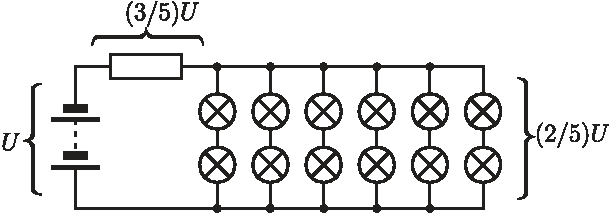
\includegraphics{2018-v2g-08-lambid-joonis}
\end{center}
b) Until all the lamps are lit each lamp will have a voltage $U/5$ where $U$ is the terminal voltage of the voltage source. The total power is respectively
\[
P_1=12\times \frac{U^2}{25R}=\frac{12U^2}{25R},
\] 
where $R$ is the resistance of a single lamp. If one of the lamps would fuse then the lamp connected sequentially to it would also stop working. We are left with only 5 chains connected in parallel and thus the total resistance of the lamps is $2R/5$. Now taking the distribution of the voltage in the diagram into consideration the power on each lamp will be
\[
U\times \frac{2R/5}{2R/5+R/2} \times \frac{1}{2}=\frac{2}{9}U
\] 
and the total power of the lamps respectively
\[
P_2=10\times \frac{4U^2}{81R}=\frac{40U^2}{81R}.
\] 
Therefore the total power increases $P_2/P_1=250/243\approx \num{1.029}$ times.\\
\emph{Note}. There are additional suitable diagrams. We will bring some examples.\\
\begin{itemize}
\item We connect the lamps in series by three and then 4 such series in parallel. In this case the total power of the lamps decreases 1.080 times in the part \emph{b)}.
\item We connect the lamps in parallel by four and then 3 such blocks in series with the resistor. In this case the total power of the lamps decreases by 1.024 times in the part \emph{b)}.
\end{itemize}
More working diagrams can be found.
\probend